Escribe una expresión para calcular el perímetro y el área de la figura \ref{fig:20230319044608}

\begin{figure}[H]
  \centering
  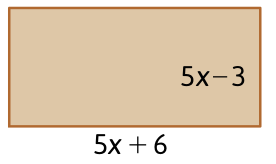
\includegraphics[width=0.25\textwidth]{../images/20230319044608}
  \caption{}
  \label{fig:20230319044608}
\end{figure}

\begin{solutionbox}{4cm}
  \begin{multicols}{2}
    Perímetro:
    \begin{align*}
      P & =2(5x+6)+2(5x-3) \\
        & =10x+12+10x-6    \\
        & =20x+6
    \end{align*}

    Área:
    \begin{align*}
      A & =(5x+6)(5x-3)     \\
        & =25x^2-15x+30x-18 \\
        & =25x^2+15x-18
    \end{align*}
  \end{multicols}
\end{solutionbox}